% Options for packages loaded elsewhere
\PassOptionsToPackage{unicode}{hyperref}
\PassOptionsToPackage{hyphens}{url}
\PassOptionsToPackage{dvipsnames,svgnames,x11names}{xcolor}
%
\documentclass[
  authoryear]{elsarticle}

\usepackage{amsmath,amssymb}
\usepackage{iftex}
\ifPDFTeX
  \usepackage[T1]{fontenc}
  \usepackage[utf8]{inputenc}
  \usepackage{textcomp} % provide euro and other symbols
\else % if luatex or xetex
  \usepackage{unicode-math}
  \defaultfontfeatures{Scale=MatchLowercase}
  \defaultfontfeatures[\rmfamily]{Ligatures=TeX,Scale=1}
\fi
\usepackage{lmodern}
\ifPDFTeX\else  
    % xetex/luatex font selection
\fi
% Use upquote if available, for straight quotes in verbatim environments
\IfFileExists{upquote.sty}{\usepackage{upquote}}{}
\IfFileExists{microtype.sty}{% use microtype if available
  \usepackage[]{microtype}
  \UseMicrotypeSet[protrusion]{basicmath} % disable protrusion for tt fonts
}{}
\makeatletter
\@ifundefined{KOMAClassName}{% if non-KOMA class
  \IfFileExists{parskip.sty}{%
    \usepackage{parskip}
  }{% else
    \setlength{\parindent}{0pt}
    \setlength{\parskip}{6pt plus 2pt minus 1pt}}
}{% if KOMA class
  \KOMAoptions{parskip=half}}
\makeatother
\usepackage{xcolor}
\setlength{\emergencystretch}{3em} % prevent overfull lines
\setcounter{secnumdepth}{5}
% Make \paragraph and \subparagraph free-standing
\ifx\paragraph\undefined\else
  \let\oldparagraph\paragraph
  \renewcommand{\paragraph}[1]{\oldparagraph{#1}\mbox{}}
\fi
\ifx\subparagraph\undefined\else
  \let\oldsubparagraph\subparagraph
  \renewcommand{\subparagraph}[1]{\oldsubparagraph{#1}\mbox{}}
\fi


\providecommand{\tightlist}{%
  \setlength{\itemsep}{0pt}\setlength{\parskip}{0pt}}\usepackage{longtable,booktabs,array}
\usepackage{calc} % for calculating minipage widths
% Correct order of tables after \paragraph or \subparagraph
\usepackage{etoolbox}
\makeatletter
\patchcmd\longtable{\par}{\if@noskipsec\mbox{}\fi\par}{}{}
\makeatother
% Allow footnotes in longtable head/foot
\IfFileExists{footnotehyper.sty}{\usepackage{footnotehyper}}{\usepackage{footnote}}
\makesavenoteenv{longtable}
\usepackage{graphicx}
\makeatletter
\def\maxwidth{\ifdim\Gin@nat@width>\linewidth\linewidth\else\Gin@nat@width\fi}
\def\maxheight{\ifdim\Gin@nat@height>\textheight\textheight\else\Gin@nat@height\fi}
\makeatother
% Scale images if necessary, so that they will not overflow the page
% margins by default, and it is still possible to overwrite the defaults
% using explicit options in \includegraphics[width, height, ...]{}
\setkeys{Gin}{width=\maxwidth,height=\maxheight,keepaspectratio}
% Set default figure placement to htbp
\makeatletter
\def\fps@figure{htbp}
\makeatother

\makeatletter
\@ifpackageloaded{caption}{}{\usepackage{caption}}
\AtBeginDocument{%
\ifdefined\contentsname
  \renewcommand*\contentsname{Table of contents}
\else
  \newcommand\contentsname{Table of contents}
\fi
\ifdefined\listfigurename
  \renewcommand*\listfigurename{List of Figures}
\else
  \newcommand\listfigurename{List of Figures}
\fi
\ifdefined\listtablename
  \renewcommand*\listtablename{List of Tables}
\else
  \newcommand\listtablename{List of Tables}
\fi
\ifdefined\figurename
  \renewcommand*\figurename{Figure}
\else
  \newcommand\figurename{Figure}
\fi
\ifdefined\tablename
  \renewcommand*\tablename{Table}
\else
  \newcommand\tablename{Table}
\fi
}
\@ifpackageloaded{float}{}{\usepackage{float}}
\floatstyle{ruled}
\@ifundefined{c@chapter}{\newfloat{codelisting}{h}{lop}}{\newfloat{codelisting}{h}{lop}[chapter]}
\floatname{codelisting}{Listing}
\newcommand*\listoflistings{\listof{codelisting}{List of Listings}}
\makeatother
\makeatletter
\makeatother
\makeatletter
\@ifpackageloaded{caption}{}{\usepackage{caption}}
\@ifpackageloaded{subcaption}{}{\usepackage{subcaption}}
\makeatother
\journal{JIMR}
\ifLuaTeX
  \usepackage{selnolig}  % disable illegal ligatures
\fi
\usepackage[]{natbib}
\bibliographystyle{elsarticle-harv}
\usepackage{bookmark}

\IfFileExists{xurl.sty}{\usepackage{xurl}}{} % add URL line breaks if available
\urlstyle{same} % disable monospaced font for URLs
\hypersetup{
  pdftitle={Data inteoperability in context: the importance of open source implementations when choosing open standards},
  pdfauthor={Daniel Kapitan; Femke Heddema; Andre Dekker; Melle Sieswerda; Bart-Jan Verhoeff},
  pdfkeywords={OMOP, OpenEHR, FHIR, secondary use, data
platform, digital platform},
  colorlinks=true,
  linkcolor={blue},
  filecolor={Maroon},
  citecolor={Blue},
  urlcolor={Blue},
  pdfcreator={LaTeX via pandoc}}

\setlength{\parindent}{6pt}
\begin{document}

\begin{frontmatter}
\title{Data inteoperability in context: the importance of open source
implementations when choosing open standards}
\author[1,2,3]{Daniel Kapitan%
%
}
 \ead{daniel@kapitan.net} 
\author[2]{Femke Heddema%
%
}

\author[4]{Andre Dekker%
%
}

\author[5,4]{Melle Sieswerda%
%
}

\author[6]{Bart-Jan Verhoeff%
%
}


\affiliation[1]{organization={Dutch Hospital
Data},city={Utrecht},country={the
Netherlands},countrysep={,},postcodesep={}}
\affiliation[2]{organization={PharmAccess
Foundation},city={Amsterdam},country={the
Netherlands},countrysep={,},postcodesep={}}
\affiliation[3]{organization={Eindhoven University of
Technology},city={Eindhoven},country={the
Netherlands},countrysep={,},postcodesep={}}
\affiliation[4]{organization={Maastricht
University},city={Maastricht},country={the
Netherlands},countrysep={,},postcodesep={}}
\affiliation[5]{organization={Integral Cancer Registry
Netherlands},city={Eindhoven},country={the
Netherlands},countrysep={,},postcodesep={}}
\affiliation[6]{organization={Expertisecentrum
Zorgalgoritmen},city={Utrecht},country={the
Netherlands},countrysep={,},postcodesep={}}

\cortext[cor1]{Corresponding author}





        
\begin{abstract}
In response to the proposal of Tsafnat et al.~to converge towards three
open health data standards, this viewpoint provides a critical
reflection on the proposed alignment of using OpenEHR, FHIR and OMOP as
the default standards for clinical care and administration, data
exchange and longitudinal analysis, respectively. We argue that open
standards are a necessary but not sufficient condition to achieve health
data interoperability. The ecosystem of open source implementations
needs to be considered when choosing an appropriate standard for a given
context. We discuss two specific contexts, namely standardization of i)
health data for federated learning, and ii) health data sharing in low-
and middle income countries (LMICs). Specific design principles,
practical considerations and implementation choices for these two
context are described, based on ongoing work in both areas. In the case
of federated learning, we observe convergence towards OMOP and FHIR,
where the two standards can effectively be used side-by-side given the
availibility of mediators between the two. In the case of health
information exchanges in LMICs, we see a strong convergence towards FHIR
as the primary standard, with as yet limited adoption of OMOP and
OpenEHR. We propose practical guidelines for context-specific adaptation
of open standards.
\end{abstract}





\begin{keyword}
    OMOP \sep OpenEHR \sep FHIR \sep secondary use \sep data
platform \sep 
    digital platform
\end{keyword}
\end{frontmatter}
    
\section{Open standards are a necessary but not sufficient condition for
interoperability}\label{open-standards-are-a-necessary-but-not-sufficient-condition-for-interoperability}

``A paradox of health care interoperability is the existence of a large
number of standards exists with significant overlap among them,'' say
Tsafnat et al., followed by a call to actions towards the health
informatics community to put effort into establishing convergence and
preventing collision \citep{tsafnat2024converge}. To do so, they propose
to converge on three open standards, namely i) OpenEHR for clinical care
and administration; ii) Fast Health Interoperability Resources (FHIR)
for data exhange and iii) Observational Medical Outcomes Partnership
Common Data Model (OMOP) for longitudinal analysis. They argue that open
data standards, backed by engaged communities, hold an advantage over
proprietary ones and therefore should be chosen as the steppingstones
towards achieving true interoperability.

While we support their high-level rationale and intention, we feel their
proposed trichotomy does not do justice to details that are crucial in
real-world implementations. This viewpoint provides a critical
reflection on their proposed framework in three parts. First, we reflect
on salient differences between the three open standards from the
perspective of the notion of openness of digital platforms
\citep{dereuver2018digital} and the paradox of open
\citep{keller2021paradox}. Subsequently, we present our findings in
designing and implementing health data platforms in two specific
contexts, namely i) platforms for federated learning on shared health
data in high income countries; and ii) health data platforms for low and
middle income countries (LMICs). We conclude with practical guidelines
for context-specific adaptation of open standards.

\section{Digital platforms require extensibility, availibility of
complementary components and availibility of executable pieces of
software}\label{digital-platforms-require-extensibility-availibility-of-complementary-components-and-availibility-of-executable-pieces-of-software}

Besides the paradox of interoperability put forward by Tsafnat et al.,
we argue that open standards are a necessary, but not sufficient
condition for convergence of health data standarization. We posit that
open source implementations of components, libraries etc. constitute
another necessary condition for establishing a flourishing health data
sharing platform and associated ecosystem for any given context, be it
regional, international or within a specific sub-domain like pandemic
preparedness. Research on digital platforms underline the importance of
the platform openness, not only in term of open standards, but also in
term of extensibility of the code base, availibility of complements to
the core technical platform (in our case the data standard itself) and
availibility of executable pieces of software
\citep{dereuver2018digital}. Only when the majority of these aspects of
digital platforms are fullfilled can we resonably expect that the
platform will indeed be longlived.

In what they call the paradox of open, Keller and Tarkowsi argue that
this conventional approach of open standards and open source flourish
under two types of conditions \citep{keller2021paradox}. First, projects
where many people contribute to the creation of a common resource have
proven succesful. ``This is the story of Wikipedia, OpenStreetMap,
Blender.org, and the countless free software projects that provide much
of the internet's infrastructure.'' \citep{keller2021paradox} Indeed,
Tsafnat et al.~have explicitly taken into account that ``an engaged and
vibrant community is a major advantage for the longevity of the data
standards it uses,'' which has informed their proposal to converge
towards OMOP, FHIR en OpenEHR. However, the emphasis on open source
implementations is somewhat overlooked. This point is only mentioned in
passing and indirectly, when Tsafnat et al.~reference work done by
Reynolds and Wyatt who already argued in 2011 ``\ldots{} for the
superiority of open source licensing to promote safer, more effective
health care information systems. We claim that open source licensing in
health care information systems is essential to rational procurement
strategy'' \citep{reynolds2011open}. We believe that a realistic
assessment of the current position of an open standard within the wider
context of availability of complementary components and open source
implementations is equally important when choosing which standard to
adopt.

This point is related to the second condition put forward by Keller and
Tarkoswki, namely that the conventional open approach has proven
fruitful when ``opening up'' is the result of external incentives or
requirements, rather than voluntary actions. ``This is the story of
publicly-funded knowledge production like Open Access academic
publications, cultural heritage collections in the Public Domain, Open
Educational Resources (OER), and Open Government data.''
\citep{keller2021paradox} A canonical example is the birth of the GSM
standard, which was mandated by European legislation.\footnote{See
  \url{https://en.wikipedia.org/wiki/GSM\#Initial_European_development}
  for details.} Reflecting on this perspective on openness, we observe a
salient difference between FHIR vis-a-vis OpenEHR and OMOP, namely that
the former is the only one that has been mandated (or at least strongly
recommended) in some jurisdictions. In the US, the Office of the
National Coordinator for Health Information Technology (ONC) and the
Centers for Medicare and Medicaid Services (CMS) has introduced a steady
stream of new regulations, criteria, and deadlines in Health IT that has
resulted in significant adoption of FHIR \citep{firely2023fhir}. In
India, the open Health Claims Exchange protocol specification - which is
based on FHIR - has been mandated by the Indian government as the
standard for e-claims handling \citep{india2020national, hcx}. The
African Union recommends all new implementations and digital health
system improvements use FHIR as the primary mechanism for data exchange
\citep{tilahun2023african}, but doesn't say anything about the use of,
for example, OpenEHR for administrative point-of-service systems.

These external incentives have resulted in a large boost in both
commercial and open source development activities in the FHIR ecosystem.
Illustrative of this is the speed with which the Bulk FHIR API has been
defined and implemented in almost all major implementations
\citep{mandl2020push, jones2021landscape}, and the the SQL-on-FHIR
specification to make large-scale analysis of FHIR data accessible to a
larger audience and portable between systems.\footnote{https://build.fhir.org/ig/FHIR/sql-on-fhir-v2/}
It has also led to more people voluntarily contributing to FHIR-related
open source projects, which has resulted in a wide offering of FHIR
components across major technology stacks (Java, Python, .NET), thereby
strengthening the first condition. By comparison, OMOP and OpenEHR have
not yet profited from external incentives to spur the adoption and
thereby growing the ecosystem beyond a certain critical mass. To
illustrate this, a search on GitHub on ``FHIR'' yields 8.2 thousand
results, ``OMOP or OHDSI'' one thousand results, and ``OpenEHR'' returns
400 results. A quick-scan of the available open source components listed
on the website of the three governing bodies HL7, OHDSI and OpenEHR,
indicates that the ecosystem of FHIR and OMOP have a significantly
larger offering of extensible and complementary open source components
than OpenEHR.\footnote{FHIR:
  https://confluence.hl7.org/display/FHIR/Open+Source+Implementations .
  OMOP: https://www.ohdsi.org/software-tools/. OpenEHR:
  https://openehr.org/products\_tools/platform/}

Hence, we stress that beyond the evaluating the instrinic structure of
an open standard and the community that supports the standard, we need
to take into account the wider ecosystem of open source implementations,
complementary components etc. From this wider perspective of the whole
ecosystem surrounding the three standards, FHIR stands out as having the
most diverse and rich ecosystem because it has been mandated in certain
jurisdictions. This is relevant when comparing these standards in
real-world implementations. We now turn to two specific use cases c.q.
contexts where these considerations are at play.

\section{Standarization of health data for federated
learning}\label{standarization-of-health-data-for-federated-learning}

The current fragmentation in health data is one of the major barriers
towards leveraging the potential medical data for machine learning (ML).
Without access to sufficient data, ML will be limited in its application
to health improvement efforts and, ultimately, from making the
transition from research to clinical practice. High quality health data,
obtained from a research setting or a real-world clinical practice
setting, is hard to obtain, because health data is highly sensitive and
its usage is tightly regulated.

Federated learning (FL) is a learning paradigm that aims to address
these issues of data governance and privacy by training algorithms
collaboratively without moving (copying) the data itself
\citep{rieke2020future, teo2024federated}. Based on ongoing work with
the PLUGIN healthcare consortium (\url{https://plugin.healthcare}, in
Dutch) we have detailed an architecture for FL for secondary use of
health data for hospitals in the Netherlands. Starting point for this
implementation are the National Health Data Infrastructure agreements
for research, policy and innovation for the Dutch healthcare sector,
which have been adopted at the beginning of 2024
\citep{healthri2024agreements}. Figure~\ref{fig-healthri-architecture}
shows a high level overview of the platform, which comprises three areas
(multiple use, applications and generic features) and a total of 26
functional components (for details please refer to
\citep{healthri2024agreements}). One of the prerequisites of this
architecture is that organizations that participate in a federation of
`data stations' use the same common data model to make the data
Findable, Accessible, Interoperable and Resusable (FAIR). These FAIR
data stations comprise components 7, 8 and 9 in
Figure~\ref{fig-healthri-architecture}, i.e.~the data, metadata and
APIs, respectively, through which this the data station can be accessed
and used.

\begin{figure}

\centering{

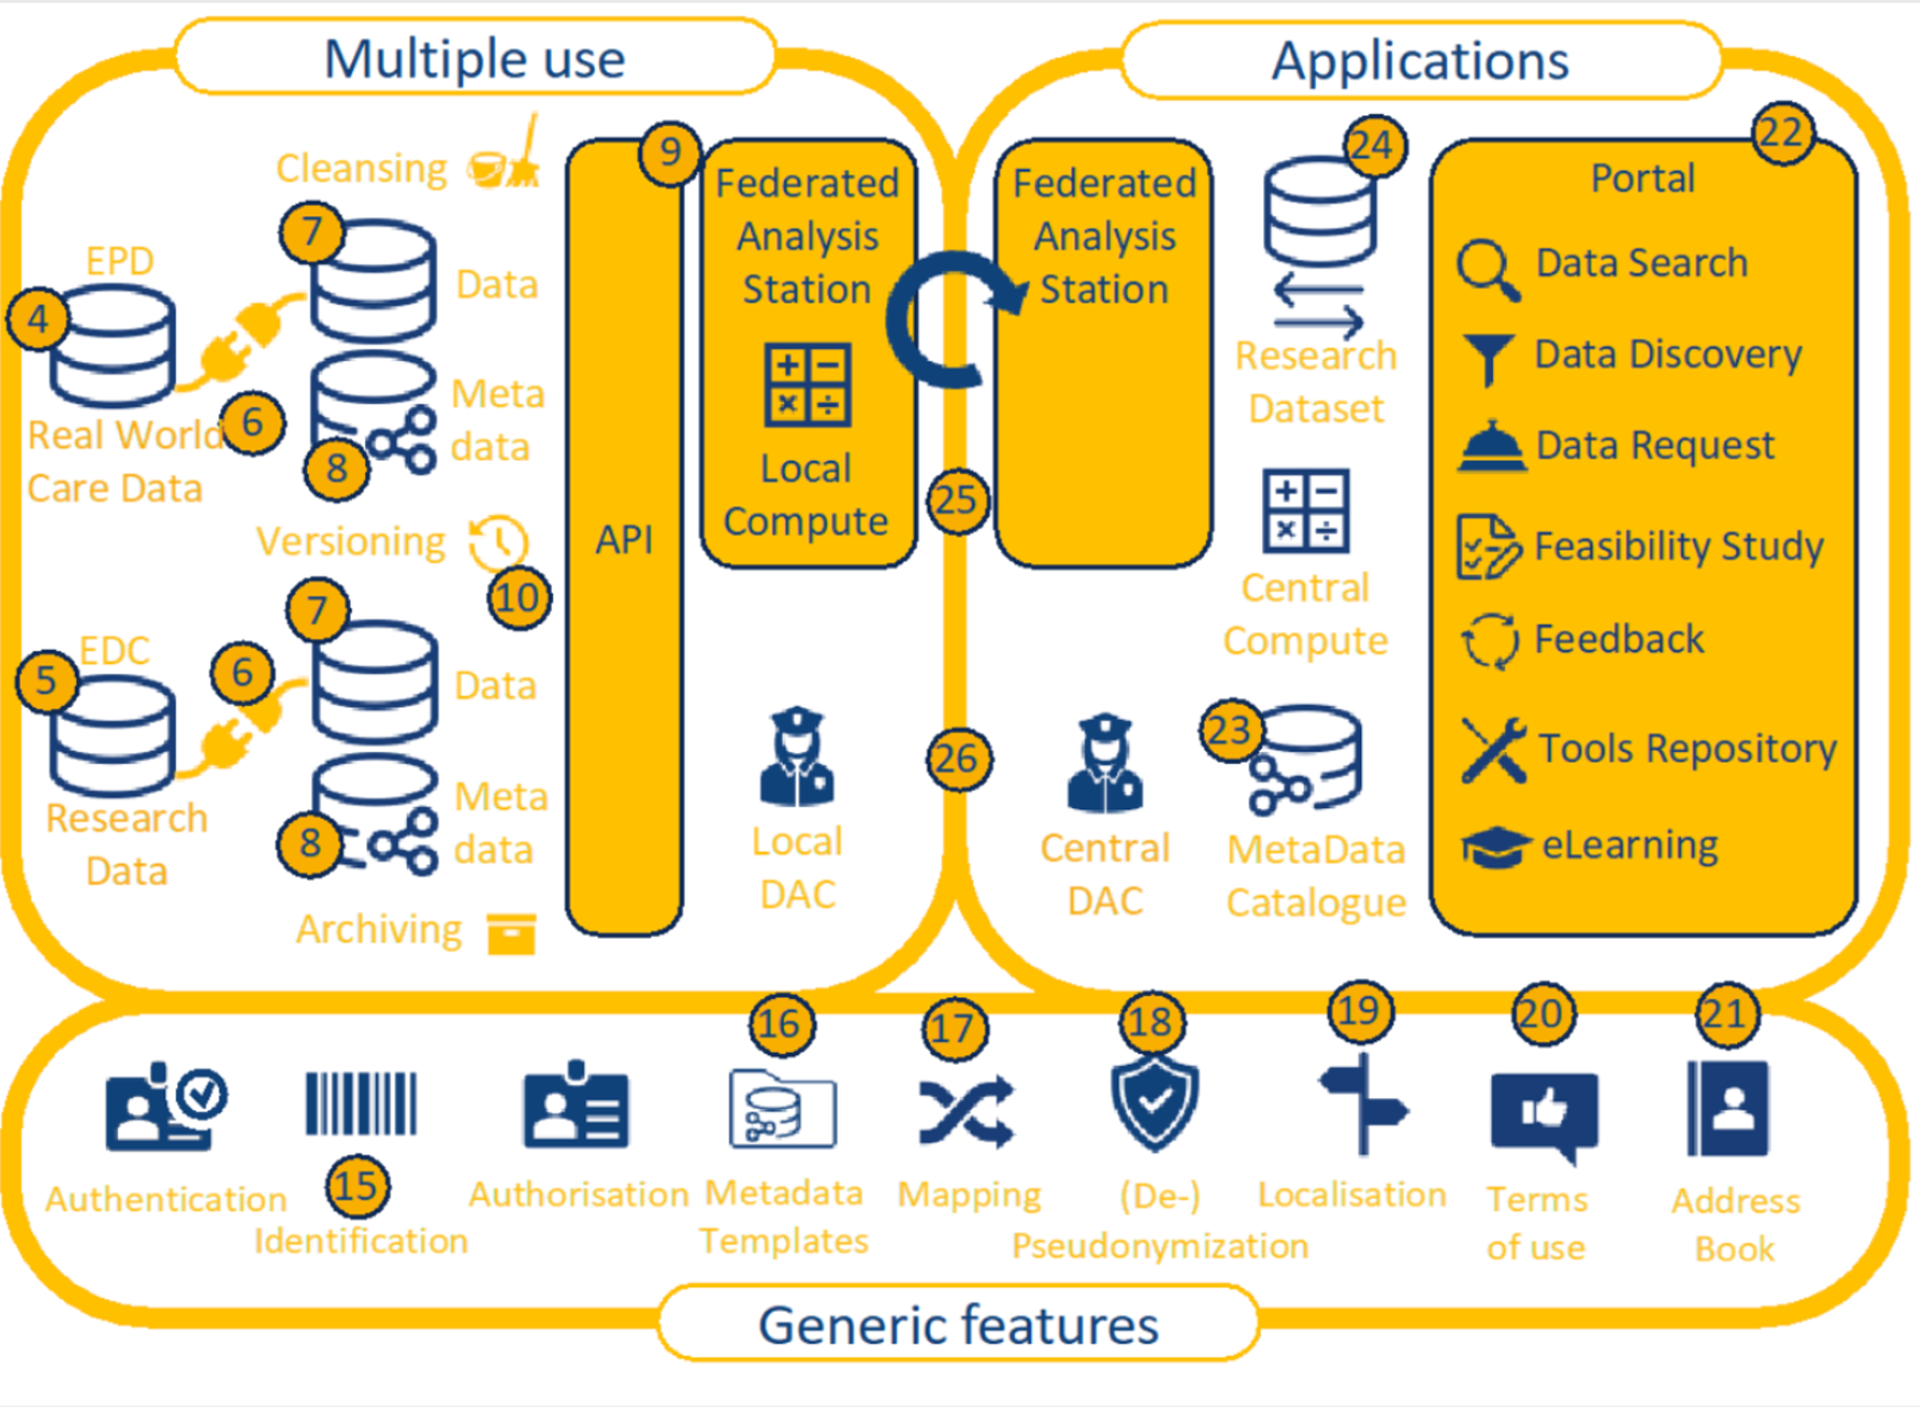
\includegraphics{health-ri-architecture.png}

}

\caption{\label{fig-healthri-architecture}Reference architecture for the
Dutch health data infrastructure for research and innovation
\citep{healthri2024agreements}}

\end{figure}%

Following the line of reasoning of Tsafnat et al., OMOP would be the
go-to standard for storing the longitudinal data in each of the data
stations. Indeed, by now there are quite a few reports of real-world
implementations of federated learning networks based on the OHDSI-OMOP
stack, including a global infrastructure with 22 centres for COVID19
prediction models\citep{khalid2021standardized}, FeederNet in South
Korea with 57 participating hospitals \citep{lee2022feedernet}, Dutch
multi-cohort dementia research with 9 centres \citep{mateus2024data},
the European severe heterogeneous asthma research collaboration
\citep{kroes2022blueprint} and the recently initiated Belgian FEIN
network {[}TO DO: add reference{]}.

For the PLUGIN project, however, we choose to adopt FHIR as the common
data model because of its practicality and extensibility to be used in a
Python-based data science stack, provenance of RESTful APIs
out-of-the-box to facilitate easy integration with the container-based
vantage6 FL framework, support of many healthcare terminologies and
flexibility through the profiling mechanims
\citep{choudhury2020personal, smits2022improved}. Increasingly, other
projects have reported the use of FHIR for persistent, longitudinal
storage for FL. The CODA platform, which aims to implement a similar FL
infrastructure in Canada, compared OMOP and FHIR and chose the latter as
it has been found to support more granular mappings required for
analytics \citep{mullie2023coda}. The fair4health project has
implemented also based on FHIR, using their own open source framework
for the federated learning infrastructure itself
\citep{sinaci2024privacypreserving}.

Given that conceptually OMOP can be viewed as a strict subset of FHIR,
hybrid solutions using OMOP and FHIR combined have also been reported,
such as the German KETOS platform \citep{gruendner2019ketos}, and the
preliminary findings from the European GenoMed4All project which aims to
connect clinical and -omics data \citep{cremonesi2023need}. A
collaboration of 10 university hospitals in Germany have shown that
standardized ETL-processing from FHIR into OMOP can achieve 99\%
conformance \citep{peng2023etlprocess}, which confirms the feasiblity of
the solution pattern where FHIR acts as an intermediate sharing standard
through which data from (legacy) systems are extracted and made
available for reuse in a common data model. One could argue that the
distiction between FHIR amd OMOP becomes less relevant if data can be
effectively stored in either standard. We are hopeful that initiatives
like https://omoponfhir.org indeed will foster convergence rather than
collision between these two standards.

In the case of PLUGIN, however, we had other considerations to choose
FHIR as the persistent storage format of the data stations. One of the
important considerations is that we found that the mechanism of FHIR
Profiles can be tied to concept of late binding commonly applied in data
lake/warehouse architectures: allow ingest of widely different sources,
and gradually add more constraints and validations as you move closer to
a specific use case. If machine learning is the primary objective for
secondary use, we want to be able to cast a wider net of relevant data,
rather than being to restrictive when ingesting the data at the start of
processing pipeline. Late binding in data warehousing is a design
philosophy where data transformation and schema enforcement are deferred
until as late as possible in the data processing pipeline, sometimes
even until query time. This approach contrasts with early binding, where
data is transformed and structured as it is ingested into the data
warehouse. This principle is visualized as concentric circles
(Figure~\ref{fig-late-binding}). The advantages of this design is that
it allows for greater flexibility. During the initial ingest of the
data, we only require the data to conform to the minimal syntactic
standard defined by the base FHIR version (R4 in the diagram). As the
data is processed, more strict checks and constrains are applied,
whereby ultimately different profiles can co-exists next to one another
(the two most inner circles), within a larger circle with fewer
strictions. This approach does not support the extension mechanism of
FHIR, so we need to be cautious if we decide to use that.

\begin{figure}

\centering{

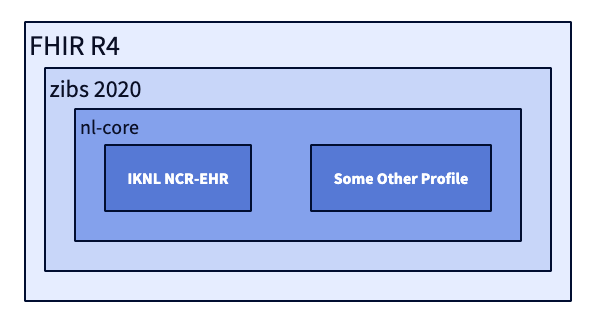
\includegraphics{late-binding.png}

}

\caption{\label{fig-late-binding}Principle of late binding with FHIR
profiling mechanism}

\end{figure}%

We found that this principle of late binding also allows flexible and
efficient implementations of the data stations that make use of the
current best practices of the a lakehouse architecture of
\citep{hai2023data, harby2022data, harby2024data} and the composable
data stack \citep{pedreira2023composable}. Lakehouses typically have a
zonal architecture that follow the Extract-Load-Transform pattern (ELT)
where data is ingested from the source systems in bulk (E), delivered to
storage with aligned schemas (L) and transformed into a format ready for
analysis (T) \citep{hai2023data}. The discerning characteristic of the
lakehouse architecture is its foundation on low-cost and
directly-accessible storage that also provides traditional database
management and performance features such as ACID transactions, data
versioning, auditing, indexing, caching, and query optimization
\citep{armbrust2021lakehouse}. Lakehouses thus combine the key benefits
of data lakes and data warehouses: low-cost storage in an open format
accessible by a variety of systems from the former, and powerful
management and optimization features from the latter.

The main disadvantage in using FHIR in this way pertains to the need for
upgrading the whole ELT pipeline when upgrading to a new primary FHIR
version, for example R5. However, we expect that the development time
required to upgrade FHIR versions is significantly less than the initial
migration to FHIR.

{[}TO DO: add more arguments here, finish this section with
conclusion/summary for this use-case{]}

\section{Health data standards in low- and middle income
countries}\label{health-data-standards-in-low--and-middle-income-countries}

It is a widely held belief that digital technologies have an important
role to play in strengthening health systems in LMICs. Yet, also here
the current fragmentation of health data stands in the way of scaling up
digital health programme beyond project-centric, vertical solutions into
sustainable health information exchanges. And also here, many have
called to converge towards open standards \citep{mehl2023fullstac}.
Based on our direct involvement in implementing and designing health
data platforms in sub-Saharan African countries, and in line with the
approach put forward by Mehl et al., we emphasis the need for
convergence not only on i) open standards, but also on ii) open
technologies (similar to our arguments discussed in the above), iii)
open architectures (doucmentation, using open standards, of reusable
enterprise architecture patterns for health systems) and iv) open
content (representations of public health, health system or clinical
knowledge to guide implementations).

Many sub-Saharan African countries have adopted the OpenHIE framework
\citep{openhie} as the architectural blueprint for implementing
nation-wide health information exchanges (HIE) \citep{mamuye2022health},
including Nigeria \citep{dalhatu2023paper}, Kenya
\citep{thaiya2021adoption} and Tanzania \citep{nsaghurwe2021one}. While
the OpenHIE specification is agnostic to which data standard should be
used, in practice the digital health community in the global South have
\emph{de facto} converged towards FHIR as the common data model, not
only for data exchange, but also for point-of-service systems to support
clinical care and administration, and persistent, longitudinal storage
of data in the so-called Shared Health Record
\citep{ohie2023unconference}. The adoption of FHIR as the default
standard for all three domains is fueled by the widespread availibility
of open-access software infrastructure which enables an end-to-end
integration. To illustrate this, consider for example, the Open Health
Stack (OHS) consists of a new suite of digital public goods, including a
software development kit for building FHIR-native apps on Android, and
analytics tooling to generate insights from FHIR data. This solution
design blurs the distinction between the three original domains for
health data standardization.

\begin{longtable}[]{@{}
  >{\centering\arraybackslash}p{(\columnwidth - 4\tabcolsep) * \real{0.1389}}
  >{\raggedright\arraybackslash}p{(\columnwidth - 4\tabcolsep) * \real{0.6111}}
  >{\raggedleft\arraybackslash}p{(\columnwidth - 4\tabcolsep) * \real{0.2500}}@{}}
\caption{Number of healthcare facilities in Kenya. Source: Kenya Health
Facility Census, Ministry of Health, September
2023.}\label{tbl-kenya-facilities}\tabularnewline
\toprule\noalign{}
\begin{minipage}[b]{\linewidth}\centering
Level
\end{minipage} & \begin{minipage}[b]{\linewidth}\raggedright
Description
\end{minipage} & \begin{minipage}[b]{\linewidth}\raggedleft
Number of facilities
\end{minipage} \\
\midrule\noalign{}
\endfirsthead
\toprule\noalign{}
\begin{minipage}[b]{\linewidth}\centering
Level
\end{minipage} & \begin{minipage}[b]{\linewidth}\raggedright
Description
\end{minipage} & \begin{minipage}[b]{\linewidth}\raggedleft
Number of facilities
\end{minipage} \\
\midrule\noalign{}
\endhead
\bottomrule\noalign{}
\endlastfoot
2 & Dispensaries and private clincs, typically located in a school,
industrial plant or other organization that dispenses medication and
sometimes basic medical and dental treatment & 8,806 \\
3 & Health centres, medium-sized units which cater for a population of
about 80,000 people & 2,559 \\
4 & Sub-county hospital, similar to health centres with additional
facilities for more complex procedures & 971 \\
5 & County referral hospital, regional centres which provide specialised
care & 34 \\
6 & National referral hospital & 5 \\
\end{longtable}

Arguments to add:

\begin{itemize}
\tightlist
\item
  explain that we don't see OpenEHR playing any role of significance.
  Largest open source EHR implementations working with own data models.
  Unlikely this will change any time soon
  \citep{syzdykova2017opensource}
\item
  instead, we see that FHIR is in fact being adopted as a
  point-of-service system. this is possible because data is of lower
  complexity and the majority of smaller health facilities are resource
  constrained anyway --\textgreater{} moving towards a scenario where an
  app used by the health care worker is the system of record. Here we
  see a convergence of the three domains put forward by Tsafnat: the
  Shared Health Record serves as the back-end of the system-of-record,
  it provides a transactional, persistent storage engine for enabling
  information exchange and it is the longitudinal data that is used
  downstream for analytics, monitoring etc.
\item
  explain example OHS/OpenSRP: maternal care
\item
  \begin{itemize}
  \tightlist
  \item
    explain there is lot of complementatry open technologies and open
    content, to get going
  \item
    and SDK to build apps
  \item
    Clinical workflows which can be configured in a FHIR-native front-
    and backend
  \item
    InstantHIE to deploy a swarm of containers to provision all relevant
    components
  \item
    leverage open source data \& analytics components to build data
    stations/data warehouses at any scle
  \end{itemize}
\item
  also technical advantages of FHIR

  \begin{itemize}
  \tightlist
  \item
    explain that because FHIR is based on web technologies, it lends it
    self serverless implementations, separation of storage and
    compute(ref composable data stack); and downward scaleability
    (running in the browser)
  \item
    how does this relate to ontologies/graph-based? FHIR can be
    expressed in graphs \citep{gebreslassie2023fhir4fair}{]}
  \end{itemize}
\item
  main disadvantages

  \begin{itemize}
  \tightlist
  \item
    FHIR profiling and versions. Still lot of work to be done prevent
    sprawl of profiles. Many LMICs still lack a standardized, national
    core profile. Inititives such as the International Patient Summary
    can be used as a stepping stone to provide arrive at a consistent
    profile for high-volume, low-complexity care such as maternal and
    antenatal care (ANC) and non-communicable diseases (NCD). In our
    experience, deployment of these HIEs have a strong focus on enabling
    primary care networks, where it makes economic sense to combine the
    SHR as a shared system-of-record of such a network.
  \end{itemize}
\end{itemize}

\begin{figure}

\begin{minipage}{\linewidth}

\begin{figure}[H]

{\centering 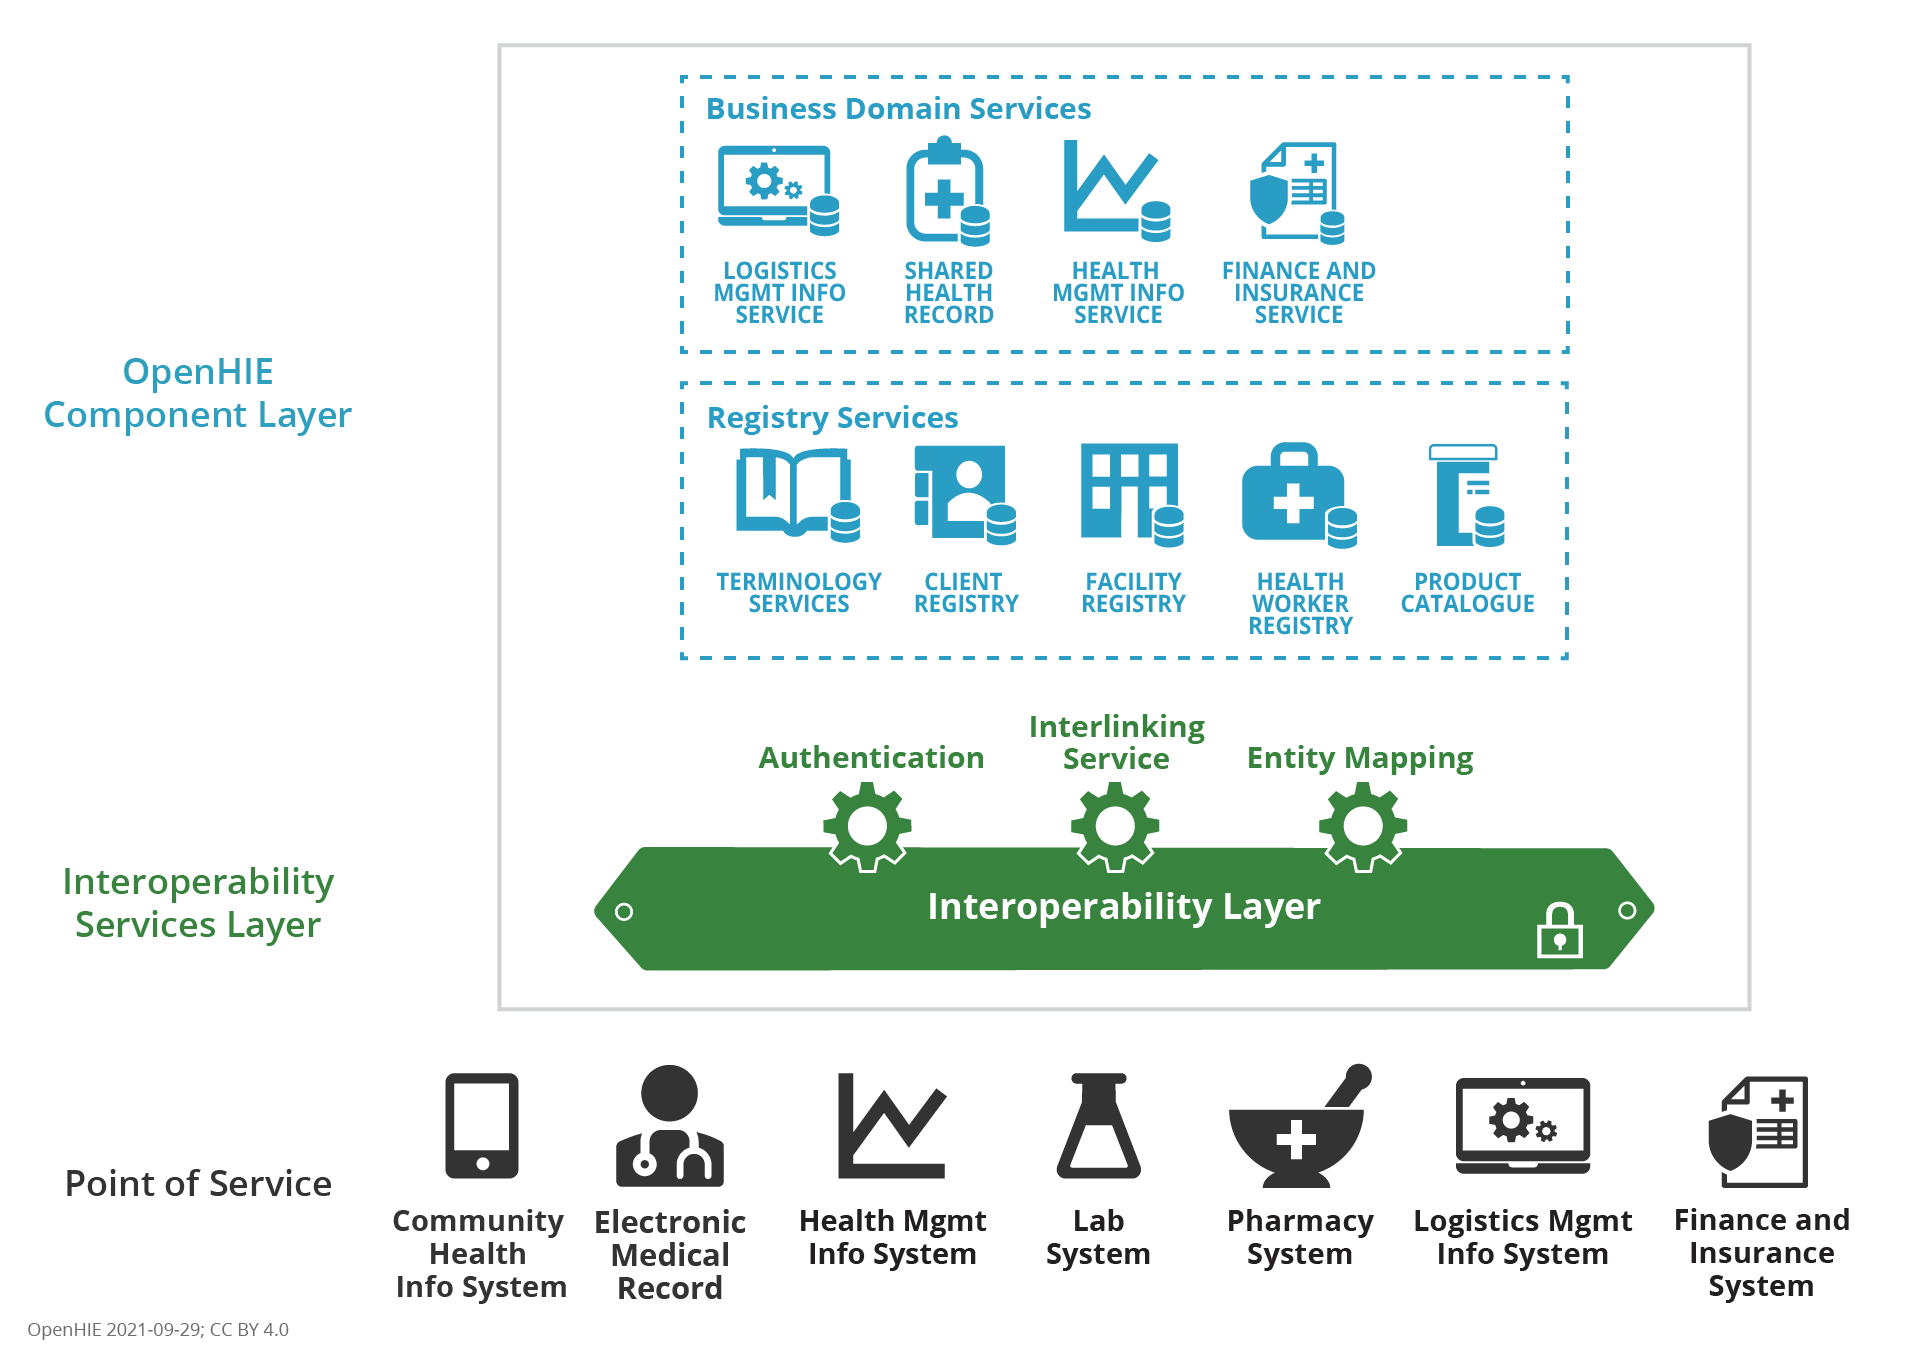
\includegraphics{openhie.png}

}

\subcaption{a)}

\end{figure}%

\end{minipage}%
\newline
\begin{minipage}{\linewidth}

\begin{figure}[H]

{\centering 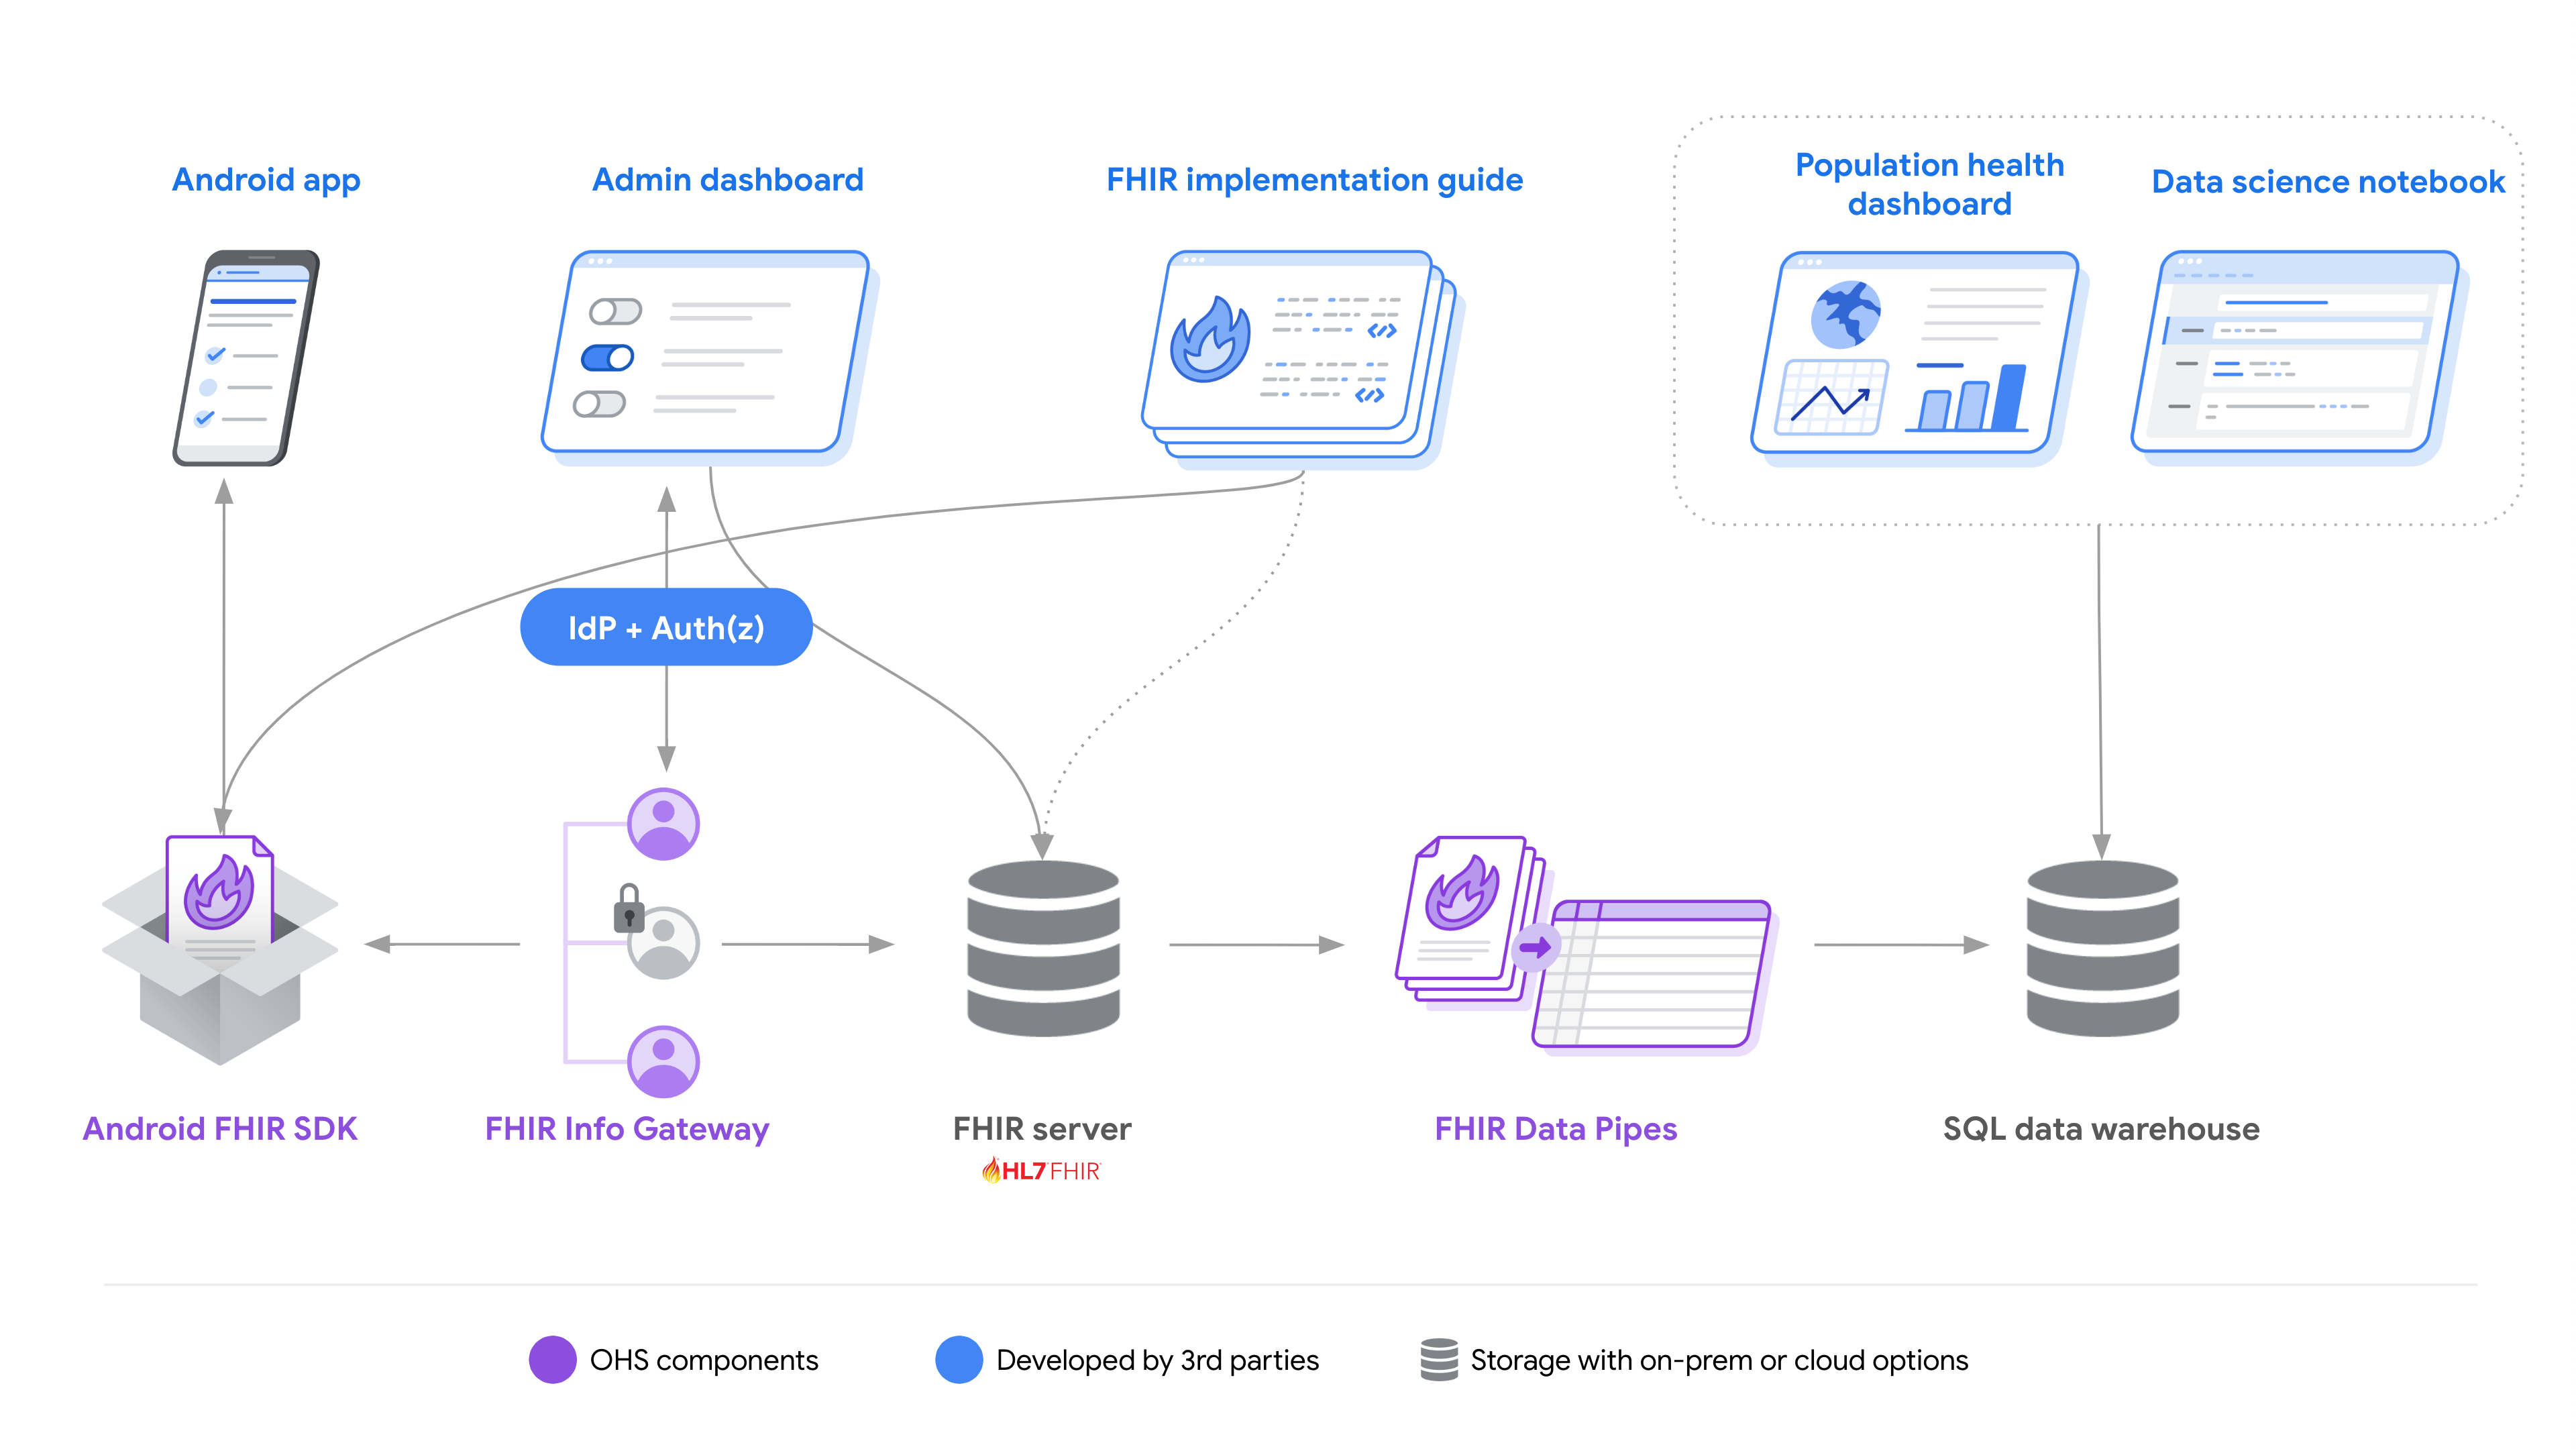
\includegraphics{ohs-endtoend.png}

}

\subcaption{b)}

\end{figure}%

\end{minipage}%

\caption{\label{fig-openhie}The OpenHIE reference architecture (a) and
themain components in the Open Health Stack (b).}

\end{figure}%

\section{Conclusion and outlook}\label{conclusion-and-outlook}

\begin{itemize}
\tightlist
\item
  We underline the need for open data standards as a necessary condition
  to achieve interoperability
\item
  It is not a sufficient condition
\item
  Suggestion: can we maken OMOP and OpenEHR benefit from the open
  technologies on FHIR? We think that through making open source
  reference implementations, such as OMOP-on-FHIR (what's EHR equivalent
  of that?) we can
\item
  MPC as next step up from FL
\item
  More than a decade later, we observe that only a very small fraction
  of health IT systems are based on open source, the majority of which
  are used in LMICs which we will discuss later
  \citep{digitalpublicgoods}.
\end{itemize}


  \bibliography{plugin.bib}


\end{document}
